%!TEX TS-program = xelatex
\documentclass[12pt, a4paper]{article}  

%%%%%%%%%%%%%%% Шрифты %%%%%%%%%%%

\usepackage[british,russian]{babel} % выбор языка для документа
\usepackage[utf8]{inputenc} % задание utf8 кодировки исходного tex файла

\usepackage{fontspec}         % пакет для подгрузки шрифтов
\setmainfont{Wilhelm Gotisch}   % задаёт основной шрифт документа

\usepackage{wrapfig}
\usepackage{graphicx}                  % Для вставки рисунков
\usepackage{graphics}
\graphicspath{/home/alex/Документы/Латекс/HW_2/images/}

%%%%%%%%%%%%%%%%%%%%%%%% Оформление %%%%%%%%%%%%%%%%%%%%%%%%%%%%%%%%%

\usepackage[paper=a4paper,top=15mm, bottom=15mm,left=35mm,right=10mm,includefoot]{geometry}
\usepackage{indentfirst}       % установка отступа в первом абзаце главы


% Заголовок
\author{ГЕРЦОГУ БЕХАРСКОМУ\\
	 МАРКИЗУ ХИБРАЛЕОНСКОМУ, \\
	 ГРАФУ БЕНАЛЬКАСАРСКОМУ И БАНЬЯРЕССКОМУ,\\ 
	 ВИКОНТУ АЛЬКОСЕРСКОМУ, СЕНЬОРУ КАПИЛЬЯССКОМУ, \\
	 КУРЬЕЛЬСКОМУ И БУРГИЛЬОССКОМУ} 
\title{ПОСВЯЩЕНИЕ}
\date{1615 год}

\begin{document}
	\maketitle 
	
	\begin{wrapfigure}{L}{0.5\linewidth}
		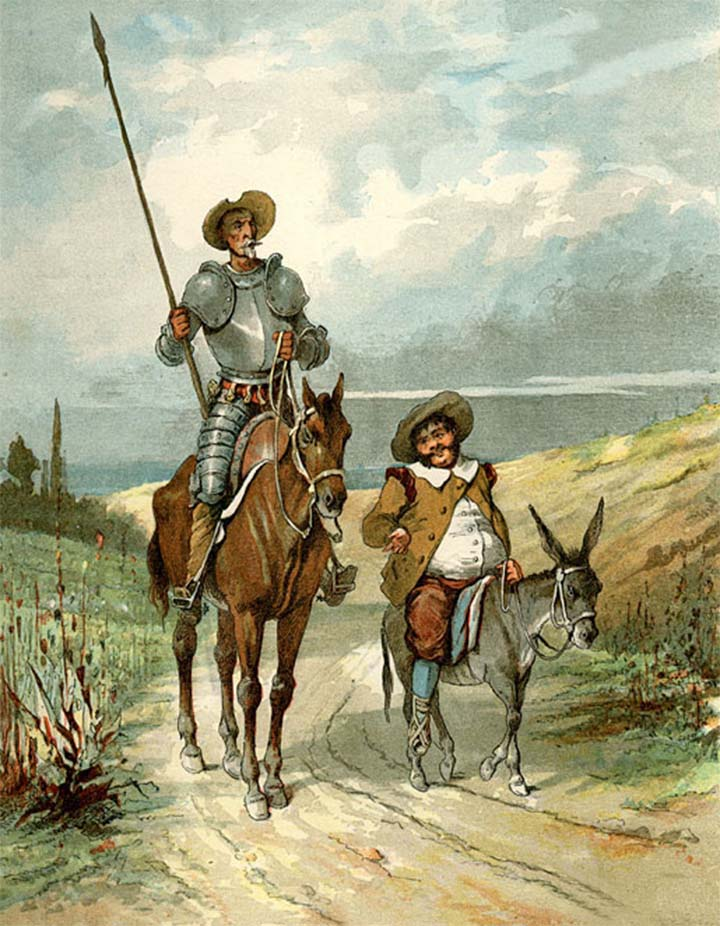
\includegraphics[width=\linewidth]{/home/alex/Документы/Латекс/HW_2/images/don-quijote-con-sancho-panza}
		\caption{Дон Кихот Ламанчский}
	\end{wrapfigure}
Ввиду того, что Вы, Ваша Светлость, принадлежа к числу  вельмож,  столь
склонных поощрять изящные искусства, оказываете радушный  и  почетный  прием
всякого рода книгам, наипаче же таким, которые  по  своему  благородству  не
унижаются до  своекорыстного  угождения  черни,  положил  я  выдать  в  свет
Хитроумного идальго Дон Кихота Ламанчского под защитой  достославного  имени
Вашей Светлости и ныне,  с  тою  почтительностью,  какую  внушает  мне  Ваше
величие, молю Вас принять его под  милостивое  свое  покровительство,  дабы,
хотя  и  лишенный  драгоценных  украшений  изящества  и   учености,   обычно
составляющих   убранство   произведений,   выходящих   из-под   пера   людей
просвещенных, дерзнул он под сенью Вашей Светлости бесстрашно  предстать  на
суд тех, кто, выходя за пределы собственного невежества,  имеет  обыкновение
при разборе чужих трудов выносить не столько справедливый,  сколько  суровый
приговор, - Вы же, Ваша Светлость, вперив очи мудрости своей  в  мои  благие
намерения, надеюсь, не отвергнете столь  слабого  изъявления  нижайшей  моей
преданности.
	
\end{document}


